\section{Task 4: Open-Set Recognition}

\subsection{Experimental Setup}
% Brief 2-3 sentence overview: CIFAR-10 as the ten known classes; CIFAR-100 used only at
% final evaluation, 100 images per unknown class. Near unknowns: bus, pickup truck,
% motorcycle, tractor, wolf, fox, leopard, camel (800 images). Far unknowns: bottle, bowl,
% chair, clock, keyboard, mushroom, sunflower, wardrobe (800 images). CIFAR ResNet-18
% (3x3 stride-1 first conv, no max-pool, 32x32 input), SGD lr 0.1 / momentum 0.9 / weight
% decay 5e-4 with cosine decay, batch 128, 100 epochs, seed 6304, checkpoint = best CIFAR-10
% validation accuracy. GCSC = same recipe + RandAugment(2 ops, magnitude 9). PROSER =
% fine-tuned from the Vanilla checkpoint for 50 epochs with 5 dummy classifiers and
% layer-2 manifold mixup (Beta(2,2)). Rejection threshold = 95th percentile of
% unknownness on CIFAR-10 validation, so about 95% of known examples are accepted.

\subsection{Semantic Similarity and Rejection}

\begin{table}[h]
  \caption{Post-hoc scores on the frozen Vanilla model: AUROC (CIFAR-10 test against each unknown group) and rejection at the threshold that accepts 95\% of CIFAR-10 validation images. Known: CIFAR-10 test images accepted. 800 images per unknown group.}
  \label{tab:task4_posthoc}
  \centering
  \small
  \setlength{\tabcolsep}{4pt}
  \begin{tabular}{lccccccc}
    \toprule
    & \multicolumn{3}{c}{\textbf{AUROC}} & & \multicolumn{3}{c}{\textbf{Rejection (\%)}} \\
    \cmidrule(lr){2-4} \cmidrule(lr){6-8}
    \textbf{Score} & Near & Far & All & Known (\%) & Near & Far & All \\
    \midrule
    MSP         & \textbf{0.814} & 0.887 & 0.850 & 94.09 & 31.38 & 46.38 & 38.88 \\
    MLS         & 0.802 & 0.883 & 0.842 & 94.22 & \textbf{34.75} & \textbf{54.13} & \textbf{44.44} \\
    Energy      & 0.802 & 0.883 & 0.843 & 94.41 & 34.50 & 53.25 & 43.88 \\
    Mahalanobis & 0.795 & \textbf{0.911} & \textbf{0.853} & 94.36 & 27.75 & 51.38 & 39.56 \\
    \bottomrule
  \end{tabular}
\end{table}



\begin{table}[h]
  \caption{Most confidently accepted near and far unknowns (Vanilla, MLS); an image is accepted when its score is below the threshold $-6.058$. Per-class acceptance: Appendix Fig.~\ref{fig:task4_unknown_classes}.}
  \label{tab:task4_failures}
  \centering
  \small
  \begin{tabular}{llcc@{\hspace{18pt}}llc}
    \toprule
    \multicolumn{3}{c}{\textbf{Near unknowns}} & & \multicolumn{3}{c}{\textbf{Far unknowns}} \\
    \cmidrule(lr){1-3} \cmidrule(lr){5-7}
    Unknown & Predicted & Score & & Unknown & Predicted & Score \\
    \midrule
    wolf          & dog        & $-12.12$ & & keyboard  & bird     & $-12.15$ \\
    fox           & cat        & $-12.04$ & & mushroom  & bird     & $-11.89$ \\
    bus           & truck      & $-11.60$ & & chair     & airplane & $-11.77$ \\
    tractor       & ship       & $-11.54$ & & keyboard  & truck    & $-11.54$ \\
    pickup truck  & automobile & $-11.46$ & & sunflower & bird     & $-11.52$ \\
    \bottomrule
  \end{tabular}
\end{table}

The semantic similarity of certain classes made the rejection substantially harder for the model. With the vanilla MLS measure of unknownness, the model rejected only \(34.75\%\) near unknowns with an AUROC of \(0.802\), whereas it rejected around \(54.13\%\) far unknowns with an AUROC of \(0.883\).

The most frequently accepted unknown classes were among pickup trucks (\(91\%\) accepted, most often as automobiles), bus (\(82\%\), most often as truck), and wolf (\(77\%\), most often as dog). Similarly, the model confused wolves as dogs and leopards as cats, indicating that the visual and semantic similarity among some of the unknown categories with known ones is quite plausible, making rejection difficult for the model.

Among some of the semantically far unknowns, the wardrobe (\(68\%\)), bowl (\(53\%\)), and sunflower (\(47\%\)) had the highest acceptance rates. Additional confident failures are the keyboard/mushroom by bird and chair by airplane. The high acceptance rates for these failed semantically far unknowns suggest that the classifier might have responded to incidental similarities in shape, color or some other spurious correlations like background rather than some discriminative class features.

\FloatBarrier
\subsection{What the Novelty Scores Capture}

\begin{figure}[t]
  \centering
  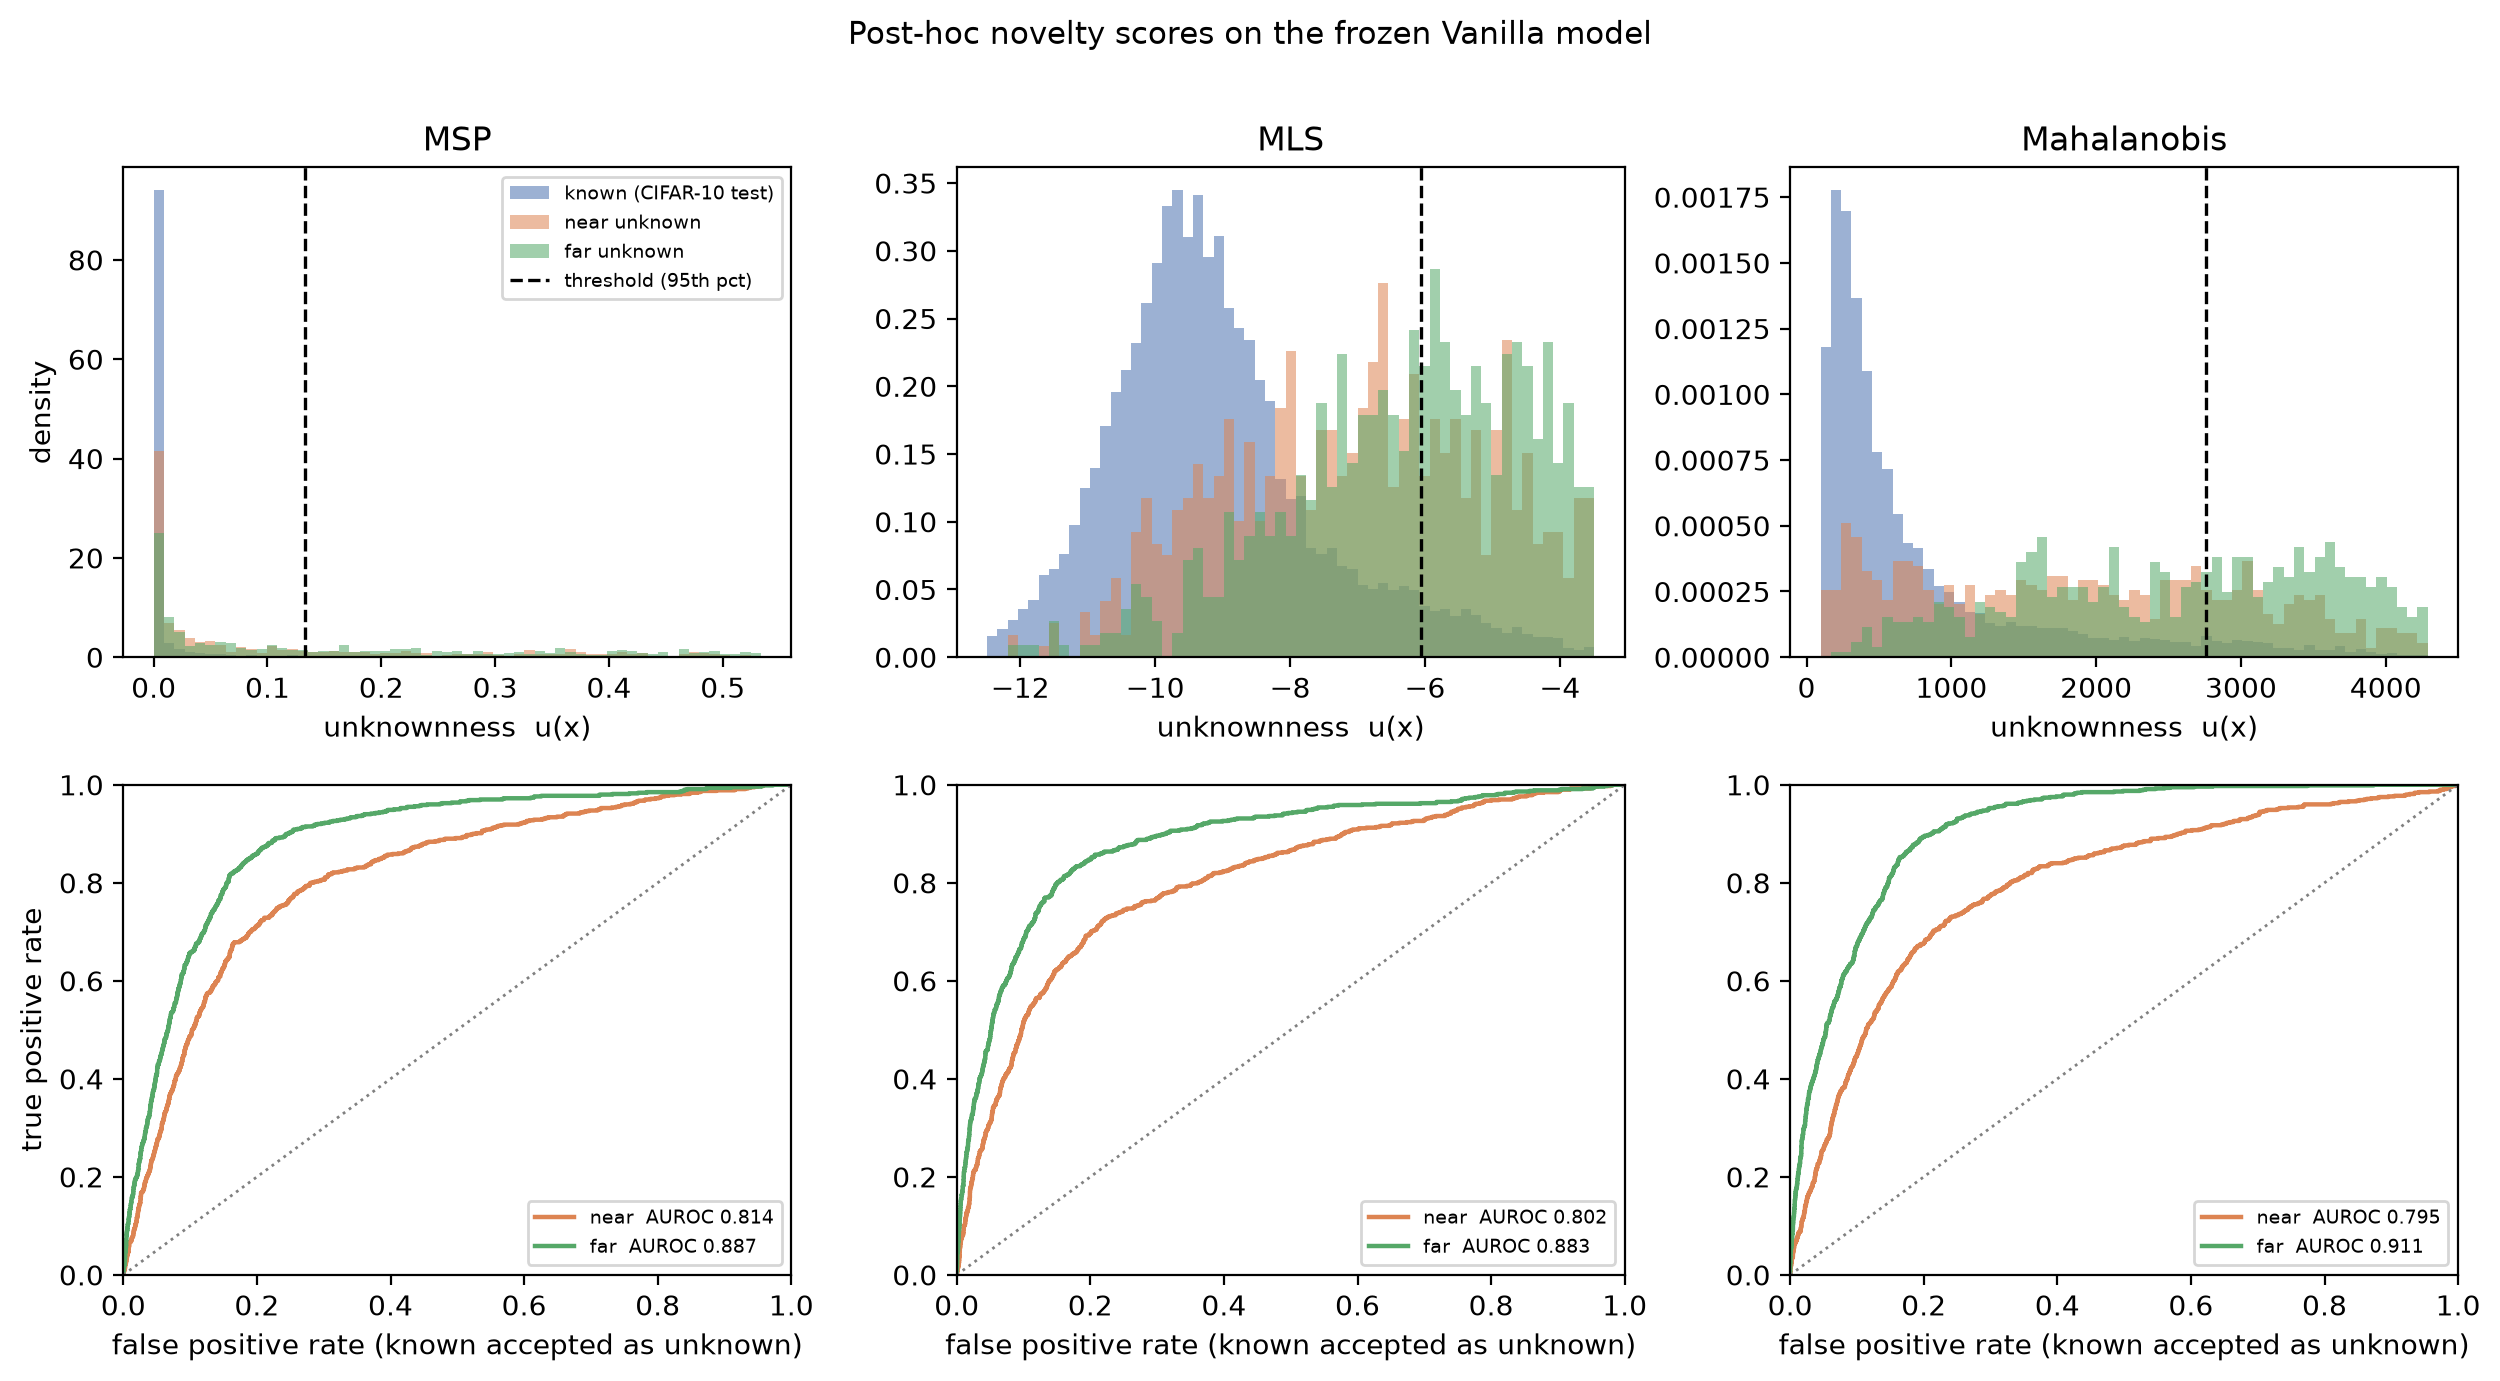
\includegraphics[width=\textwidth]{figures/task4/fig1_osr_scores.png}
  \caption{MSP, MLS and Mahalanobis on Vanilla. Top: unknownness distributions with the threshold (dashed). Bottom: ROC curves for known against near and far unknowns.}
  \label{fig:task4_scores}
\end{figure}

MSP measures relative softmax confidence, where the dominant probability is considered as known-like, and the probabilities spread across classes are unknowns. Given as
MSP unknownness is:
\[ u_{\mathrm{MSP}}(x) = 1-\max_kp_k(x). \]
As compared to MSP, MLS measures the largest absolute logit. The maximum logit represents the strongest raw response of the classifier among the known classes. Given as:

\(u_{\mathrm{MLS}}(x) = -\max_kz_k(x).\)

Here, the negative sign makes the largest value the smallest, representing strength of unknownness: the smaller the \(u_{\mathrm{MLS}}(x)\) the more known the class is.
Where MSP and MLS uses the max single value to compute the unknownness, Energy uses all the classifier logits to compute unknownness, given as:

\[ u_{\mathrm{Energy}}(x) = -\log \sum_{k=1}^{K}e^{z_k(x)}. \]
For CIFAR-10:
\[ K=10. \]
The expression:
\[ \log\sum_ke^{z_k} \]
is called logsumexp.
For large known-class logits, it produces a large total known-class response, which, through the negative, becomes smaller; the small energy means more known.
Mahalanobis measures distance from the nearest known-class feature cluster by calculating a shared diagonal covariance from the training features
For each class:
\[ D_c(x) = (f(x)-\mu_c)^T \Sigma^{-1} (f(x)-\mu_c). \]
Because the covariance is diagonal, this becomes:
\[ D_c(x) = \sum_{j=1}^{512} \frac{ (f_j(x)-\mu_{c,j})^2 }{ \sigma_j^2+\epsilon }. \]
And Mahalanobis novelty score is given as:

\(u_{\mathrm{Mah}}(x) = \min_cD_c(x).\)
I.e., if the feature f(x) is close to at least one known class cluster, the score will be small; otherwise, large.

Novelty scores for all four methods show that classifying far unknowns as unknown was much easier than near unknowns; MLS and energy methods produced almost identical results \(0.802/0.883\) and \(0.802/0.883\) near/far AUROC. This indicates that the largest logit dominated. MSP was most effective for near unknowns, with the highest AUROC of  \(0.814\), which indicates that the relative probability has marginally more information for semantically similar unknowns.

Mahalanobis produced the best far AUROC (\(0.911\)) and the best overall AUROC (\(0.853\)) as well. It shows that for semantically far classes, the feature distance was particularly informative. However, on the contrary, it depicted the weakest near rejection because the near unknowns lie closer to the known clusters, as in the case of wolves and buses, which can lie close to dog or vehicle feature clusters.

Therefore, MSP softmax confidence was most useful for ranking near unknowns, feature distance was strongest for far unknowns, and using all logits through Energy added little beyond MLS in this experiment.

\FloatBarrier
\subsection{Did GCSC Improve Closed-Set and Open-Set Performance?}

\begin{table}[h]
  \caption{Vanilla, GCSC and PROSER with MLS, plus PROSER's placeholder score. CSA uses the ten known-class logits; rejection as in Table~\ref{tab:task4_posthoc}.}
  \label{tab:task4_models}
  \centering
  \small
  \setlength{\tabcolsep}{3.5pt}
  \begin{tabular}{lcccccccc}
    \toprule
    & & \multicolumn{3}{c}{\textbf{AUROC}} & & \multicolumn{3}{c}{\textbf{Rejection (\%)}} \\
    \cmidrule(lr){3-5} \cmidrule(lr){7-9}
    \textbf{Model (score)} & CSA (\%) & Near & Far & All & Known (\%) & Near & Far & All \\
    \midrule
    Vanilla (MLS)            & 94.54 & 0.802 & 0.883 & 0.842 & 94.22 & 34.75 & 54.13 & 44.44 \\
    GCSC (MLS)               & \textbf{95.12} & \textbf{0.826} & \textbf{0.909} & \textbf{0.868} & 94.60 & \textbf{37.13} & \textbf{59.00} & \textbf{48.06} \\
    PROSER (MLS)             & 94.63 & 0.803 & 0.887 & 0.845 & 94.64 & 32.75 & 50.00 & 41.38 \\
    PROSER (placeholder)     & 94.63 & 0.780 & 0.886 & 0.833 & 94.91 & 29.88 & 48.25 & 39.06 \\
    \bottomrule
  \end{tabular}
\end{table}

GCSC shows a slight improvement on closed-set performance, where it gained 0.58 points over the vanilla model, which is about 58 images out of 10,000 test images, not a big number. Since we used only one seed for the dataset, this improvement is not something on which we can assert the claim that GCSC improves the closed-set performance. On open-set, the ordered ranking score AUROC on near and far shows a tiny improvement of 0.024 and 0.027, respectively.

While the AUROC gains were roughly the same for both near and far unknowns, at the rejection threshold for near and far unknowns model reports a gain of 2.38 points on near unknown rejections and 4.88 points on far unknown rejections. This suggests that the augmentation might have encouraged a kind of representation that is less dependent on superficial fluctuations in appearances and thus improved known-class recognition and detection of unknowns. However, the augmentation still does not fully resolve the semantic overlap between classes like bus and truck or wolf and dog, and near-semantic novelty remains the harder problem.

\FloatBarrier
\subsection{Did PROSER Improve Rejection, and What Was the CSA Trade-off?}

The PROSER method via MLS reported an AUROC of 0.845, a 0.003 increase over Vanilla (0.842); however, it's still below GCSC (0.868) by 0.023. It reports near and far rejection rates as \(32.75\%\) and \(50.00\%\) respectively, on the lower side compared to both Vanilla \(34.75\%/54.13\%\) and GCSC \(37.13\%/59.00\%\). The closed-set accuracy of \(94.63\%\) is roughly same as of Vanilla (\(94.54\%\)) and GCSC (\(95.12\%\)).

PROSER's own placeholder scores were also weaker, especially on near unknowns compared to MLS, with an AUROC of 0.780 on near and 0.886 on far, and rejection rates of \(29.88\%\) and \(48.25\%\), respectively. The PROSER was fine-tuned for 50 epochs; however, the highest validation accuracy was achieved very early at the 4th epoch, which may explain why the placeholders were weaker, as at that moment the placeholders' loss was still relatively high; thus, the dummy classifiers had not yet learned stronger class boundaries. Later training did reduce the placeholders' loss; however, it destabilized the validation accuracy, which dropped it as low as 53.12\% at epoch 13 and ended at 93.40\% at epoch 50, below the 95.20\% best.

The models' reported results were not strong enough to clearly support the claim that the classifier and the data placeholders tightened the decision boundaries usefully. The interpolation between the known classes appears insufficient to represent the actual near and far unknown distributions. The model reported several confident failures, such as bus/truck and fox/cat, suggesting that the near unknown lies close to a single known class rather than between two knowns. On the other hand, the failures, such as the keyboard/bird and chair/airplane, show that far unknowns may also occupy directions not represented by interpolating known-class features.
